\def\year{2017}\relax
%File: formatting-instruction.tex
\documentclass[letterpaper]{article}

\usepackage{graphicx}
\usepackage{amsmath}
\usepackage{amssymb}
\usepackage{amsthm,mathrsfs,amsfonts,dsfont}
\usepackage{algorithm}
\usepackage{algorithmic}
\usepackage{threeparttable}
\usepackage{multirow}
\usepackage{subfigure}
\usepackage{color}
\usepackage{bm}
%\usepackage[vlined,boxed,ruled]{algorithm2e}
\usepackage{url}
\usepackage{xspace}

\newtheorem{corollary}{Corollary}
\newtheorem{definition}{Definition}
\newtheorem{theorem}{Theorem}
\newtheorem{proposition}{Proposition}
\newtheorem{lemma}{Lemma}
\newtheorem{remark}{Remark}



\usepackage{aaai17}
\usepackage{times}
\usepackage{helvet}
\usepackage{courier}


\def\bE{{\bf E}}
\def\blambda{{\bm \lambda}}
\def\calL{{\mathcal{L}}}
\def\bL{{\bf L}}
\def\bO{{\bf O}}
\def\bU{{\bf U}}
\def\bV{{\bf V}}
\def\dsR{\mathds{R}}
\def\bX{{\bf X}}
\def\bx{{\bf x}}
\def\btx{{\tilde{\bf x}}}
\def\by{{\bf y}}
\def\bw{{\bf w}}
\def\btw{{\tilde{\bf w}}}
\def\tK{\tilde{K}}
\def\txi{\tilde{\xi}}
\def\tildeb{{\tilde{b}}}
\def\tphi{{\tilde{\phi}}}
\def\bz{{\bf z}}
\def\br{{\bf r}}
\def\bv{{\bf v}}
\def\bb{{\bf b}}
\def\bp{{\bf p}}
\def\bA{{\bf A}}
\def\bI{{\bf I}}

\def\bx{{\bf x}}
\def\bX{{\bf X}}
\def\by{{\bf y}}
\def\bY{{\bf Y}}
\def\bw{{\bf w}}
\def\bW{{\bf W}}
\def\balpha{{\bm \alpha}}
\def\bmu{{\bm \mu}}
\def\bK{{\bf K}}
\def\bg{{\bf g}}
\def\bp{{\bf p}}
\def\p{p}
\def\bP{{\bf P}}

\def\balpha{{\bm \alpha}}
\def\bbeta{{\bm \beta}}
\def\eg{{\emph{e.g.}}}

\def\ttTP{{\tt TP}}
\def\ttFP{{\tt FP}}
\def\ttFN{{\tt FN}}

\def\st{{\text{s.t.}}}
\def\rank{{\text{rank}}}

\def\yanred{\textcolor{red}}
\def\yanblue{\textcolor{blue}}


\frenchspacing
\setlength{\pdfpagewidth}{8.5in}
\setlength{\pdfpageheight}{11in}
\pdfinfo{
/Title (Insert Your Title Here)
/Author (Put All Your Authors Here, Separated by Commas)}
\setcounter{secnumdepth}{0}
 \begin{document}


% The file aaai.sty is the style file for AAAI Press
% proceedings, working notes, and technical reports.
%



\title{Maximum Margin Matrix Factorization for Ensemble Clustering}

%\author{AAAI Press\\
%Association for the Advancement of Artificial Intelligence\\
%2275 East Bayshore Road, Suite 160\\
%Palo Alto, California 94303\\
%}



\maketitle



\begin{abstract}
In this paper, we propose an efficient maximum margin matrix factorization algorithm for ensemble clustering.
Our contributions include i) introduction of an efficient optimization for matrix completion based ensemble clustering methods; ii) an intuitive motivation for a $\ell_{2,1}$ loss.
\end{abstract}






\section{Introduction}

A single clustering result could be inaccurate, so some researchers study ensemble clustering methods to boost the performance,
such as the algorithms proposed in~\cite{yiicdm2012robust,gaoijcai2016robust}, to name a few.

The key aim of matrix completion based methods is to detect the anomalous clusters (bad partitions/assigments) and reconstruct the real assignments,
which is shown in Figure~\ref{fig:anomalous_cluster}.
A typical formulation of matrix completion based methods then can be written as below:
\begin{align}\label{eq:typical_mc}
  \min_{\bX} ~&~ || \bX - \bL ||_2^2   \nonumber \\
  \st        ~&~ \rank(\bX) \leq k  ,
\end{align}
\noindent
where $k$ is a pre-defined rank constraint,
and $\bL \in \dsR^{N \times MK}$.
Here we denote $M$ and $K$ as the number of single clustering assignments and the number of clusters, respectively.
However, the least square loss used in matrix completion is sensitive to the abnormal errors, namely outliers, the not appropriate to capture the anomalous assignments.
The authors in~\cite{gaoijcai2016robust} propose to achieve cluster-wise (column-wise) sparsity of $\bX$ by the $\ell_{2,1}$ norm on $\bX$, which is as follow
\begin{align}\label{eq:mc_l21_gaospaper}
  \min_{\bX} ~&~ || \bL - \bX ||_F^2 + \beta || \bX ||_{2,1}   \nonumber \\
  \st        ~&~ \rank(\bX) \leq k   ,
\end{align}
\noindent
where $|| \bX ||_{2,1} = \sum_{j = 1}^{MK} \sqrt(\sum_{i=1}^{N}) = \sum_{j=1}^{MK} || \bX_{.j} ||_2$,
which would make some columns of $\bX$ as zeros (beware the direction of the computation of the $\ell_{2,1}$ norm, more details in~\cite{nienips2010efficient}).
Nevertheless, it does not consider the outliers in their loss function.
In fact, the term $|| \bL - \bX ||_F^2$ is sensitive to outliers, and the term $|| \bX ||_{2,1}$ is equivalent to $|| \bX - \bO ||_{2,1}$, which makes $\bX$ fit $\bO$, where $\bO$ is a matrix with all entries as zero.
Therefore, we propose to apply $\ell_{2,1}$ to capture the outliers as well as anomalous columns, which can be written as below
\begin{align}\label{eq:mc_l21}
  \min_{\bX} ~&~ || \bL - \bX ||_{2,1}    \nonumber \\
  \st        ~&~ \rank(\bX) \leq k  .
\end{align}
Problem~(\ref{eq:mc_l21}) is NP-hard due to the presence of the low rank constraint.
For the sake of efficiency on large scale matrices, we consider matrix factorization approaches to optimize it, which can be written as
\begin{align}\label{eq:mf_l21}
  \min_{\bX} ~&~ || \bL - \bX ||_{2,1}    \nonumber \\
  \st        ~&~ \bX = \bU \bV,~\bU \in \dsR^{N \times k},~\bV \in \dsR^{k \times MK} .
\end{align}
\noindent
Note that we have totally $K$ single clustering assignments.
Intuitively, we could set $k = K$ in Problem~(\ref{eq:mf_l21}).
Most existing matrix factorization optimization methods only consider smooth loss functions,
but the $\ell_{2,1}$ loss in Problem~(\ref{eq:mf_l21}) is nonsmooth.
In this paper, we apply augmented Lagrangian multiplier (ALM) to optimize the nonsmooth objective function efficiently.



\section{ALM Optimization}

By introducing a new variable $\bE = \bL - \bX$, we can develop Problem~(\ref{eq:mf_l21}) as below:
\begin{align}\label{eq:mf_l21_constrained}
  \min_{\bE, \bX} ~&~ || \bE ||_{2,1}   \nonumber \\
  \st             ~&~ \bE = \bL - \bX   \nonumber \\
                  ~&~ \bX = \bU \bV,~\bU \in \dsR^{N \times k},~\bV \in \dsR^{k \times MK}
\end{align}
The augmented Lagrangian function of Problem~(\ref{eq:mf_l21}) is as below
\begin{align}\label{eq:lagrangian_l21}
  \calL = || \bE ||_{2,1} + \blambda^{\top} (\bX - \bL + \bE) + \frac{\mu}{2} || \bX - \bL + \bE ||_F^2   ,
\end{align}
\noindent
where $\bX = \bU \bV$,
and $\blambda$ are the Lagrangian multipliers (or dual variables).
Then we could update $\bX$ and $\bE$ alternatively.


Specifically, to update $\bX$, we consider the following problem:
\begin{align}\label{eq:problem_X}
  \min_{\bX} ~&~ \blambda^{\top} (\bX - \bL + \bE) + \frac{\mu}{2} || \bX - \bL + \bE ||_F^2  \nonumber  \\
  \st        ~&~ \bX = \bU \bV,~\bU \in \dsR^{N \times k},~\bV \in \dsR^{k \times MK}   .
\end{align}
Problem~(\ref{eq:problem_X}) includes a smooth loss function w.r.t. $\bX$, thus can be solved by a standard matrix factorization method, such as~\cite{yanijcai2015scalable,tanicml2014riemannian,vandereyckensiamjo2013low}.


Problem~(\ref{eq:problem_X}) can also be rewritten as below
\begin{align}\label{eq:problem_X2}
  \min_{\bX} ~&~ \frac{\mu}{2} \Big( || \bX - \bL + \bE ||_F^2 + \frac{2}{\mu} \blambda^{\top} (\bX - \bL + \bE) + \frac{|| \blambda ||_F^2}{\mu^2} \Big)    \nonumber   \\
             ~&~ - \frac{\mu}{2} \frac{|| \blambda ||_F^2}{\mu^2}   \nonumber \\
  \st.       ~&~ \bX = \bU \bV,~\bU \in \dsR^{N \times k},~\bV \in \dsR^{k \times MK}   .
\end{align}
\noindent
We can obtain the final problem w.r.t. $\bX$:
\begin{align}\label{eq:problem_X3}
  \min_{\bX} ~&~ || \bX - \bL + \bE + \frac{\blambda}{\mu} ||_F^2   \nonumber \\
  \st        ~&~ \bX = \bU \bV,~\bU \in \dsR^{N \times k},~\bV \in \dsR^{k \times MK}   .
\end{align}
\noindent
There are a number of optimization algorithms for Problem~(\ref{eq:problem_X3}), such as LRGeomCG\footnote{\yanred{Code available at~\url{http://www.unige.ch/math/vandereycken/matrix_completion.html}}}.





To update $\bE$, we consider the following problem:
\begin{align}\label{eq:problem_E}
  \yanred{
  \min_{\bE} ~ || \bE ||_{2,1} + \blambda^{\top} (\bX - \bL + \bE) + \frac{\mu}{2} || \bX - \bL + \bE ||_F^2   .
  }
\end{align}
\noindent
The above problem could be solved by the algorithm proposed in~\cite{nienips2010efficient,yangijcai2011l21}.
\yanred{Yan Yan: I am working on this optimization algorithm.}



\section{An Option on Loss Function: Max Margin}

In fact, the assignments $\bL$ contains only $0/1$ values (discrete ordinal values).
This fits the setting in~\cite{yanijcai2015scalable} very much.
It could be a contribution, since maximum margin loss achieves better performance on discrete ordinal values.
\yanred{Note: we may leave this extension as a journal?}



\section{Another Option on Loss Function: $\ell_{2,1}$ to $\ell_1$ loss}

$ell_{2,1}$ loss could be difficult to optimize.
A simple way is to replace $\ell_{2,1}$ to $\ell_1$, which would be much easier.


\begin{figure}
  \centering
  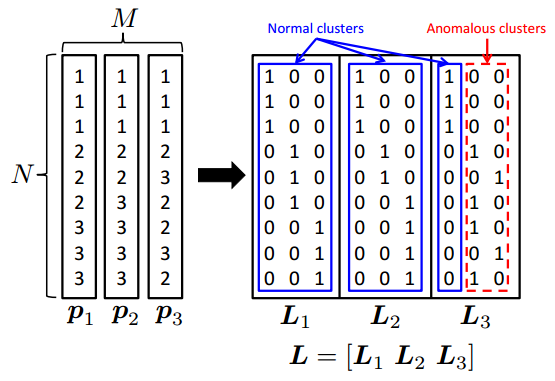
\includegraphics[width=0.49\textwidth]{anomalous_clusters.png}
  \caption{An example of anomalous cluster assignments which is retrieved from~\cite{gaoijcai2016robust}}\label{fig:anomalous_cluster}
\end{figure}







\begin{quote}
\begin{small}
  \bibliographystyle{aaai}
  \bibliography{ensemble_clustering}
\end{small}
\end{quote}

\end{document}
